\documentclass[11pt,a4paper]{article}

\usepackage[utf8]{inputenc}
\usepackage[T1]{fontenc}
\usepackage{amsmath}
\usepackage{amssymb}
\usepackage{graphicx}
\usepackage{booktabs}
\usepackage{tikz}
\usepackage[colorlinks=true,linkcolor=blue,citecolor=blue,urlcolor=blue]{hyperref}

\usetikzlibrary{arrows.meta, positioning}

\title{A Short Benchmark Note on Iterated Averages}
\author{OverBranch Benchmark Corpus\\
  \texttt{article/main.tex}}
\date{\today}

\begin{document}

\maketitle

\begin{abstract}
  We present a small, self-contained article used as a baseline workload for
  the OverBranch compiler benchmark. The document exercises common features of
  a standard \LaTeX{} article: sectioning, displayed mathematics, lists,
  tables, a schematic drawing, and cross-references. Its compile time is
  dominated by ordinary typesetting rather than by any heavy package.
\end{abstract}

\section{Introduction}\label{sec:intro}

Averages of sequences appear throughout applied mathematics. Given a sequence
$(x_n)_{n\ge 1}$, the \emph{running mean} is
\begin{equation}\label{eq:running}
  \bar{x}_n \;=\; \frac{1}{n}\sum_{k=1}^{n} x_k .
\end{equation}
Section~\ref{sec:method} describes how we iterate this operation, and
Section~\ref{sec:results} reports the observed behaviour. The notation used
throughout is summarised below.

\begin{itemize}
  \item $\mathbb{N}$ denotes the natural numbers, starting at $1$.
  \item $\|\cdot\|$ denotes the Euclidean norm on $\mathbb{R}^d$.
  \item $\mathcal{O}(\cdot)$ has its usual meaning as $n\to\infty$.
\end{itemize}

\section{Method}\label{sec:method}

Define the iterated average operator $T$ on finite sequences by
\begin{equation}\label{eq:operator}
  (Tx)_n \;=\; \frac{x_n + x_{n+1}}{2}, \qquad n \ge 1 .
\end{equation}
Applying $T$ repeatedly $m$ times yields a binomial smoothing kernel. The
coefficients of $T^m$ are given by
\begin{equation}\label{eq:binomial}
  (T^m x)_n \;=\; \sum_{j=0}^{m} \binom{m}{j} 2^{-m} x_{n+j},
\end{equation}
which follows from a straightforward induction on $m$. The table below lists
the variance reduction factor $\sigma^2(T^m x)/\sigma^2(x)$ for i.i.d.\ inputs.

\begin{table}[ht]
  \centering
  \begin{tabular}{rcl}
    \toprule
    $m$ & Kernel weights & Variance factor \\
    \midrule
    1 & $(\tfrac12,\tfrac12)$ & $\tfrac12$ \\
    2 & $(\tfrac14,\tfrac12,\tfrac14)$ & $\tfrac38$ \\
    3 & $(\tfrac18,\tfrac38,\tfrac38,\tfrac18)$ & $\tfrac{5}{16}$ \\
    4 & $(\tfrac1{16},\tfrac14,\tfrac38,\tfrac14,\tfrac1{16})$ & $\tfrac{35}{128}$ \\
    \bottomrule
  \end{tabular}
  \caption{Variance reduction of the iterated average for i.i.d.\ inputs.}
  \label{tab:variance}
\end{table}

Table~\ref{tab:variance} shows that the variance factor decreases with $m$.

\section{Schematic of the pipeline}\label{sec:pipeline}

Figure~\ref{fig:pipeline} is a schematic of the processing pipeline. It is
drawn directly in TikZ so that the document has no external dependencies.

\begin{figure}[ht]
  \centering
  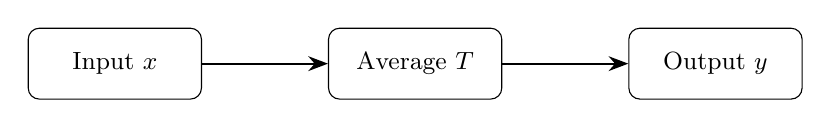
\begin{tikzpicture}[node distance=1.6cm, every node/.style={font=\small}]
    \node[draw, rounded corners, minimum width=2.2cm, minimum height=0.9cm] (in)  {Input $x$};
    \node[draw, rounded corners, minimum width=2.2cm, minimum height=0.9cm, right=of in]  (avg) {Average $T$};
    \node[draw, rounded corners, minimum width=2.2cm, minimum height=0.9cm, right=of avg] (out) {Output $y$};
    \draw[-{Stealth[length=2.5mm]}, thick] (in) -- (avg);
    \draw[-{Stealth[length=2.5mm]}, thick] (avg) -- (out);
  \end{tikzpicture}
  \caption{Processing pipeline: input, iterated averaging, output.}
  \label{fig:pipeline}
\end{figure}

\section{Results}\label{sec:results}

The variance factors in Table~\ref{tab:variance} agree with the closed form
\begin{equation}\label{eq:closed}
  \frac{\sigma^2(T^m x)}{\sigma^2(x)} \;=\; \binom{2m}{m}4^{-m},
\end{equation}
as can be checked from Equation~\eqref{eq:binomial}. For instance, at $m=2$
the right-hand side equals $\binom{4}{2}/16 = 3/8$, matching the table. The
same calculation shows that the factor tends to zero like $\mathcal{O}(m^{-1/2})$.

In summary, the iterated average is a simple and effective smoother, and its
behaviour is fully determined by the closed form above.

\section{Conclusion}

We have described an iterated averaging operator, verified a closed form for its
variance reduction, and illustrated the pipeline. The document is intentionally
modest in size, and serves as a fast-to-compile reference point.

\end{document}
